\documentclass[12pt]{article}
\usepackage{amsmath}

% we use kwarc.bib
\usepackage[backend=biber]{biblatex}
\addbibresource{kwarc.bib}

\usepackage{hyperref}
\usepackage[dvipsnames]{xcolor}
\usepackage[show]{ed}

% listings syntax highlighting for JSOn
\usepackage{listings}

\colorlet{bool}{red}
\colorlet{string}{blue}
\colorlet{number}{orange}
\colorlet{comment}{OliveGreen}
\colorlet{type}{purple}

\lstset{
    basicstyle=\small\ttfamily,
    columns=fullflexible,
    % strings
    string=[s]{"}{"},
    stringstyle=\color{string},
    % booleans
    keywords={true,false},
    keywordstyle=\color{bool},
    % comments
    comment=[s]{/*}{*/},
    morecomment=[l]{//},
    commentstyle=\color{comment},
    % types
    morekeywords=[2]{base64string,omel,uri,name,any,string,integer,decimalInteger,hexInteger,float,decimalFloat,hexFloat,byte,OMFOREIGN,OMV,attvar},
    keywordstyle=[2]{\color{type}},
}

% digits
\lstset{literate=%
   *{0}{{{\color{number}0}}}1
    {1}{{{\color{number}1}}}1
    {2}{{{\color{number}2}}}1
    {3}{{{\color{number}3}}}1
    {4}{{{\color{number}4}}}1
    {5}{{{\color{number}5}}}1
    {6}{{{\color{number}6}}}1
    {7}{{{\color{number}7}}}1
    {8}{{{\color{number}8}}}1
    {9}{{{\color{number}9}}}1
    {e-}{{{\color{number}e-}}}2
    {-}{{{\color{number}-}}}1
    {.}{{{\color{number}.}}}1
    {base64string}{{{\color{type}base64string}}}{12}%keyword gets caught by number, so escape it
}


\title{A Proposal for an OpenMath JSON Encoding\\OpenMath workshop CICM 2018}
\author{Michael Kohlhase \and Tom Wiesing}

\begin{document}
    \maketitle

    \begin{abstract}
        OpenMath is a semantic representation of mathematical objects. 

        There are several encodings of OpenMath Objects, most notably the XML and Binary encodings. 
        JSON is a lightweight data-interchange format that is present natively in many programming languages. 
        
        A few OpenMath JSON encodings already exist, which all have their advantages and disadvantages. 
        These commonly correspond to a naive representation of the XML encoding and thus do not make use of some of the features that JSON offers. 
        
        In this paper we propose a new OpenMath JSON encoding, which combines the advantages of the above. 
    \end{abstract}

    \ednote{Need to make introduction + conclusion flow better}
    \ednote{Styling the paper/citation style?}

    \section{Introduction}

OpenMath is a semantic representation of mathematical objects. \ednote{Is this OK?}
Because this paper is submitted to the OpenMath workshop, we will assume that reader is familar with OpenMath and will not introduce it further here. 

JSON \ednote{cite json}, short for \textbf{J}ava\textbf{S}cript \textbf{O}bject \textbf{N}otation, is a lightweight data-interchange format. 
While being a subset of JavaScript, it is defined independently. 
JSON can represent both primitive types and composite types.

Primitive JSON types are strings (e.g. \lstinline{"Hello world"}), Numbers (e.g. \lstinline{42} or \lstinline{3.14159265}), Booleans (\lstinline{true} and \lstinline{false}) and \lstinline{null}. 
Composite JSON types are either (non-homogeneous) arrays (e.g. \lstinline{[1, "two", false]}) or key-value pairs called objects (e.g. \lstinline|{"foo": "bar", "answer": 42}|). 

Constructs corresponding to JSON objects are found in most programming languages. 
Futhermore, the syntax is very simple; hence many languages have built-in facilities for translating their existing data structures to and from JSON. 
The use for an OpenMath JSON encoding is clear: It would enable easy use of OpenMath across many languages. 

There are existing approaches for encoding OpenMath as JSON. 
We will discuss two particular ones here. 

\paragraph{XML as JSON}
The JSONML standard \ednote{cite http://www.jsonml.org/} allows generic encoding of arbitrary XML as JSON. 
This can easily be adapted to the case of OpenMath. 
To encode an OpenMath object as JSON, one first encodes it as XML and then makes use of JSONML in a second step. 
Using this method, the term $\mathrm{plus}(x, 5)$ would correspond to: 
\begin{lstlisting}
[
    "OMOBJ",
    {"xmlns":"http://www.openmath.org/OpenMath"},
    [
        "OMA",
        [
            "OMS", 
            {"cd": "arith1", "name": "plus"}
        ],
        [
            "OMV", 
            {"name": "x"}
        ],
        [
            "OMI", 
            "5"
        ]
    ]
]
\end{lstlisting}

This translation has the advantage that it is near-trivial to translate between the XML and JSON encodings of OpenMath. 
It also has some disadvantages: 

\begin{itemize}
    \item The encoding does not use the native JSON datatypes. 
    One of the advantages of JSON is that it can encode most basic data types directly, without having to turn the data values into strings. 
    To encode the floating point value \lstinline{1e-10} (a valid JSON literal) using the JSONML encoding, one can not directly place it into the result. 
    Instead, one has to turn it into a string first.   
    Despite many JSON implementations providing such a functionality, in practice this would require frequent translation between strings and high-level datatypes.  
    This is not what JSON is intended for, instead the provided data types should be used. 

    \item The akwardness of some of the XML encoding remains. 
    Due to the nature of XML the XML encoding sometimes needs to introduce elements that do not directly correspond to any OpenMath objects. 
    For example, the \textit{OMATP} element is used to encode a set of attribute / value pairs. 
    This introduces unnecessary overhead into JSON, as an array of values could be used instead. 

    \item Many languages use JSON-like structures to implement structured data types. 
    Thus it stands to reason that an OpenMath JSON encoding should also provide a schema to allow languages to implement OpenMath easily. This is not the case for a JSONML encoding. 
\end{itemize}

\paragraph{OpenMath-JS}
The openmath-js \ednote{cite https://github.com/lurchmath/openmath-js} encoding takes a different approach. 
It is an (incomplete) implementation of OpenMath in JavaScript and was developed by Nathan Carter for use with Lurch Math on the web. 
It is written in literate coffee script, a derivative language of JavaScript. 

In this encoding, the term $\mathrm{plus}(x, 5)$ would correspond to: 
\begin{lstlisting}
{  
   "t":"a",
   "c": [  
      {  
         "t":"sy",
         "cd":"arith1",
         "n":"plus"
      },
      {  
         "t":"v",
         "n":"x"
      },
      {  
         "t":"i",
         "v":"5"
      }
   ]
}
\end{lstlisting}

This encoding solves some of the disadvantages of the JSONML encoding, however it still has some drawbacks:

\begin{itemize}
    \item It was written as a JavaScript, not JSON, encoding.
    The existing library provides JavaScript functions to encode OpenMath objects. 
    However, the resulting JSON has only minimal names. 
    This makes it difficult for humans to read and write directly. 

    \item No formal schema exists, like in the JSONML encoding. 
\end{itemize}


\ednote{Re-formulate this}Given these disadvantages, it makes sense to instead create a new OpenMath-JSON encoding. 
This encoding should combine the advantages of the above two. 

In particular, it should be close to the XML encoding, and at the same time make use of native JSON concepts. 
Furthermore, we want to formalize this encoding, which is not achieved by any existing approach, and thus enable easy validation. 
    \section{The OpenMath-JSON encoding}\label{sec:encoding}

To formalize our encoding, we decided to use JSON Schema~\cite{handrewsjsonschema:18}. 
This defines a vocabulary allowing us to validate and annotate JSON documents. 
Additionally, tools for programatic verification exist in many languages. 

Unfortunately, JSON schema is often tedious to write and read for humans. 
This is especially true when it comes to recursively defined data structures.
OpenMath has many recursive structures.
Instead of writing our encoding in JSON Schema directly, we decided to write the schema in a different language and then compile it to JSON Schema. 

For this purpose, we decided to make use of TypeScript~\cite{typescript:webpage}. 
TypeScript is a language derived from JavaScript -- TypeScript files are JavaScript plus type annotations. 
As such, it can be easily written and understood by humans. 
On top of typescript, we make use of a compiler~\cite{vega-ts-jscon-schema-generator:webpage} from TypeScript definitions into JSON Schema. 

\subsection{Encoding Details}

In general, objects in our encoding look similar to the following:
\\\begin{minipage}{\linewidth}\begin{lstlisting}
{
    "kind": "OMV",
    "id": "something",
    "name": "x"
}
\end{lstlisting}\end{minipage}

The \texttt{kind} attribute specifies which kind of OpenMath object this is. 
These values correspond to the element names used in the XML encoding. 
This correspondence lays the foundations of easy translation between the two. 
In TypeScript this property is also referred to as a \textit{Type Guard}, because if \textit{guards} the type of object that is represented. 

Like in the XML encoding it is possible to make use of structure sharing. 
For this purpose the \texttt{id} attribute can be used. 
We will come back to this in more detail below, when we define to the \texttt{OMR} type.

In the following we will go over the details of our encoding. 
For this we will make use of a TypeScript-like syntax, that is easily readable. 
In our description we omit the \texttt{id} attribute, which can be added to any encoded object. 
The complete source code of our encoding -- and details on how to use it -- can be found on Github~\cite{URL:openmathjson:github}. 

\subsubsection{Object Constructor -- OMOBJ}

The OpenMath Object Constructor -- \texttt{OMOBJ} -- is defined as follows:
\\\begin{minipage}{\linewidth}\begin{lstlisting}
{
    "kind": "OMOBJ",
    /** optional version of openmath being used */
    "openmath"?: "2.0",
    /** the actual object */
    "object": omel /* any element */
}
\end{lstlisting}\end{minipage}
Concretely, the integer 3 encapsulated in an object constructor using this encoding is as follows:
\\\begin{minipage}{\linewidth}\begin{lstlisting}
{
    "kind": "OMOBJ",
    "openmath": "2.0",
    "object": {
        "kind": "OMI", 
        "integer": 3
    }
}
\end{lstlisting}\end{minipage}

Let us have a look at this first example attribute for attribute. 

The first attribute -- \texttt{kind} -- represents the type of OpenMath object in question. 
Notice that it occurs twice -- once in the \texttt{OMOBJ} and a second time in the wrapped \texttt{OMI}. 
We will talk in detail about integer representation below, and hence only care about this first one. 

The second attribute -- \texttt{openmath} -- is defined as optional by our schema. 
This indicates the version of OpenMath that is being used -- \lstinline{"2.0"} in our case. 

The third and final attribute is the \texttt{object} attribute. 
This contains the wrapped object -- it is defined as of \texttt{omel} type. 
This type \texttt{omel} can contain any OpenMath element -- concretely
primitive objects (Symbols \texttt{OMS}, Variables \texttt{OMV}, Integers \texttt{OMI}, Floats \texttt{OMF}, Bytes \texttt{OMB}, Strings \texttt{OMSTR}), 
complex elements (Application \texttt{OMA}, Attribution \texttt{OMATTR}, Binding \texttt{OMBIND}) or
Errors \texttt{OME} and References \texttt{OMR}. 
In this particular case, we just have the integer $3$. 

\subsubsection{Symbols -- OMS}

An OpenMath Symbol is encoded as follows:
\\\begin{minipage}{\linewidth}\begin{lstlisting}
{
    "kind": "OMS",
    /** the base for the cd, optional */
    "cdbase"?: uri, /* any valid URI */, 
    /** content dictonary the symbol is in, any uri */
    "cd": uri,
    /** name of the symbol */
    "name": name /* any valid symbol name */
}
\end{lstlisting}\end{minipage}

Notice the \texttt{uri} and \texttt{name} types in the definition. 
These are not directly JSON types. 
We define the \texttt{uri} type to be a any JSON string that represents a valid URI. 
Similarly, we define the \texttt{name} type to be any JSON string that represents a valid symbol name. 

For example to encode the \texttt{sin} symbol from the \texttt{transc1} CD:
\\\begin{minipage}{\linewidth}\begin{lstlisting}
{
    "kind": "OMS",
    "cd": "transc1",
    "name": "sin"
}
\end{lstlisting}\end{minipage}

\subsubsection{Variables -- OMV}

An OpenMath Variable is encoded as follows:
\\\begin{minipage}{\linewidth}\begin{lstlisting}
{
    "kind": "OMV",
    /** name of the variable */
    "name": name
}
\end{lstlisting}\end{minipage}

We again make use of the \texttt{name} type here. 

For example to encode a variable $x$:
\\\begin{minipage}{\linewidth}\begin{lstlisting}
{
    "kind": "OMV",
    "name": "x"
}
\end{lstlisting}\end{minipage}

\subsubsection{Integers -- OMI}

Unlike the previous elements, our encoding allows integers to be encoded in three different ways. 
In particular, we define them as follows:
\\\begin{minipage}{\linewidth}\begin{lstlisting}
{
    "kind": "OMI",
    //
    // exactly one of the following
    //

    /* any json integer */
    "integer": integer,
    /* any string matching ^-?[0-9]+$ */
    "decimal": decimalInteger,
    /* any string matching ^-?x[0-9A-F]+.$ */
    "hexadecimal": hexInteger
}
\end{lstlisting}\end{minipage}

We allows integers to be represented as one of the following:
\begin{description}
    \item[JSON Integers]
    Representing an OpenMath Integer as a JSON integer allows making use of datatypes that JSON offers. 
    This was one of the goals we wanted to achieve with our encoding. 
    
    JSON has no integer type in and of itself -- it only provides a \texttt{number} type. 
    To work around this in our schema, we define a custom integer type as any number that is an integer. 
        
    OpenMath integers can be of arbitrary size. 
    While the JSON specification does not limit the size of numbers, it also allows any implementation the freedom to pick some limit. 
    Thus for reasonably sized integers, this representation works well. 
    But for larger numbers, the other two variants should be used. 

    \item[Decimal Strings]
    A second way to encode an OpenMath Integer is to make use of the straightforward decimal string encoding. 
    This is any string consisting only of digits (and potentially having a minus sign in the case of a negative integer). 

    \item[Hexademical String]
    We can allow to encode an OpenMath Integer as a hexadecimal integer. 
    To make this different from decimally encoded integers, we require a lower-case x to be placed before the string. 
    This also has the advantage that this corresponds exactly to the XML encoding.     
\end{description}

We can thus encode the integer $-120$ in three different ways:
\begin{itemize}
    \item as a JSON integer
\\\begin{minipage}{\linewidth}\begin{lstlisting}
{
    "kind": "OMI",
    "integer": -120
}
\end{lstlisting}\end{minipage}
    \item as a decimal-encoded string
\\\begin{minipage}{\linewidth}\begin{lstlisting}
{
    "kind": "OMI",
    "decimal": "-120"
}
\end{lstlisting}\end{minipage}
    \item as a hexadecimal-encoded string
\\\begin{minipage}{\linewidth}\begin{lstlisting}
{
    "kind": "OMI",
    "hexadecimal": "-x78"
}
\end{lstlisting}\end{minipage}
\end{itemize}

\subsubsection{Floats -- OMF}

Like integers, we allow floats to be encoded in three different ways:
\\\begin{minipage}{\linewidth}\begin{lstlisting}
{
    "kind": "OMF",

    //
    // exactly one of the following
    //

    /* any json number */
    "float": number,
    /* any string matching 
        (-?)([0-9]+)?(\.[0-9]+)?([eE](-?)[0-9]+)? */
    "decimal": decimalFloat,
    /* any string matching ^([0-9A-F]+)$ */
    "hexadecimal": hexFloat 
}
\end{lstlisting}\end{minipage}

Here, the different cases work exactly like in the integer case. 

We can represent a float either as a native JSON number, a string in decimal representation or a string in hexadecimal representation. 
Just like above, the string representations correspond to the ones allowed by the XML encoding. 

For example the floating point number $10^{-10}$ can be represented in three different ways:
\begin{itemize}
    \item as a JSON float
\\\begin{minipage}{\linewidth}\begin{lstlisting}
{
    "kind": "OMF",
    "float": 1e-10
}
\end{lstlisting}\end{minipage}
    \item as a decimal-encoded string
\\\begin{minipage}{\linewidth}\begin{lstlisting}
{
    "kind": "OMF",
    "decimal": "0.0000000001"
}
\end{lstlisting}\end{minipage}
    \item as a hexadecimal-encoded string
\\\begin{minipage}{\linewidth}\begin{lstlisting}
{
    "kind": "OMF",
    "hexaecimal": "3DDB7CDFD9D7BDBB"
}
\end{lstlisting}\end{minipage}
\end{itemize}

\subsubsection{Bytes -- OMB}

Bytes can be encoded in two different ways:
\\\begin{minipage}{\linewidth}\begin{lstlisting}
{
    "kind": "OMB",
    //
    // exactly one of the following
    //

    /** an array of bytes
        where a byte is an integer from 0 to 255 */
    "bytes": byte[],
    /** a base64 encoded string */
    "base64": base64string
}
\end{lstlisting}\end{minipage}

\begin{description}
    \item[Array of bytes]
    This encoding again makes use of JSON data structures -- representing bytes as a concrete list of bytes.
    As the byte datatype does not exist directly in JSON, we represent a single byte as an integer between 0 and 255 (inclusive). 

    \item[Base64 encoded string]
    A base64-encoded string of bytes corresponds to the XML encoding. 
\end{description}

For example we can encode the ascii bytes of the string \textit{hello world}
\begin{itemize}
    \item as a byte array
\\\begin{minipage}{\linewidth}\begin{lstlisting}
{
    "kind": "OMB",
    "bytes": [
        104, 101, 108, 108, 111, 32, 
        119, 111, 114, 108, 100
    ]
}
\end{lstlisting}\end{minipage}
    \item as a base64-encoded string
\\\begin{minipage}{\linewidth}\begin{lstlisting}
{
    "kind": "OMB",
    "base64": "aGVsbG8gd29ybGQ="
}
\end{lstlisting}\end{minipage}
\end{itemize}

\subsubsection{Strings -- OMS}
The encoding of strings is straightforward -- we can make use of native JSON strings. 
\\\begin{minipage}{\linewidth}\begin{lstlisting}
{
    "kind": "OMSTR", 
    /** the string */
    "string": string
}
\end{lstlisting}\end{minipage}

Thus the string \lstinline{"Hello world"} is encoded as follows:
\\\begin{minipage}{\linewidth}\begin{lstlisting}
{
    "kind": "OMSTR", 
    "string": "Hello world"
}
\end{lstlisting}\end{minipage}

\subsubsection{Applications -- OMA}

OpenMath Applications are encoded as follows:
\\\begin{minipage}{\linewidth}\begin{lstlisting}
{
    "kind": "OMA", 
    /** the base for the cd, optional */
    "cdbase"?: uri, 
    /** the term that is being applied */
    "applicant": omel, 
    /** the arguments that the applicant 
        is being applied to. Optional and
        assumed to be empty if omitted */
    "arguments"?: omel[]
}
\end{lstlisting}\end{minipage}

Here we again make use of the already known \texttt{omel} and \texttt{uri} types. 

For example when encoding $\sin(x)$ we get:
\\\begin{minipage}{\linewidth}\begin{lstlisting}
{
    "kind": "OMA",
    "applicant": {
        "kind": "OMS",
        "cd": "transc1",
        "name": "sin"
    },
    "arguments": [{
        "kind": "OMV",
        "name": "x"
    }]
}
\end{lstlisting}\end{minipage}

\subsubsection{Attributions -- OMATTR}

OpenMath Attributions are encoded as follows:
\\\begin{minipage}{\linewidth}\begin{lstlisting}
{
    "kind": "OMATTR", 
    /** the base for the cd, optional */
    "cdbase": uri, 
    /** attributes attributed to this object, non-empty */
    "attributes": ([
        OMS, omel|OMFOREIGN
    ])[],
    /** object that is being attributed */
    "object": omel
}
\end{lstlisting}\end{minipage}

Note that each attribute is represented as a pair of the name of the attribute and its corresponding value. 
This gives us the attributes property in the definiton above being an array of pairs. 
Here we have a somewhat significant derivation from the XML encoding. 
This introduced an extra element \texttt{OMATTVAR} to represent the pairs -- this is not necessary for our case. 

As an example, to attribute a variable $x$ as having real type:
\\\begin{minipage}{\linewidth}\begin{lstlisting}
{
    "kind": "OMATTR",
    "attributes": [
        [
            { "kind": "OMS", "cd": "ecc", "name": "type" },
            { "kind": "OMS", "cd": "ecc", "name": "real" }
        ]
    ],
    "object": {
        "kind": "OMV",
        "name": "x"
    }
}
\end{lstlisting}\end{minipage}

\subsubsection{Bindings -- OMB}

We encode bindings as:
\\\begin{minipage}{\linewidth}\begin{lstlisting}
{
    "kind": "OMBIND", 
    /** the base for the cd, optional */
    "cdbase"?: uri, 
    /** the binder being used */
    "binder": omel,
    /** the variables being bound, non-empty */
    "variables": (OMV | attvar)[],
    /** the object that is being bound */
    "object": omel
}
\end{lstlisting}\end{minipage}

Here, the \texttt{variables} property is defined as a non-empty array of
\begin{itemize}
    \item a variable \texttt{OMV}, or
    \item an attributed variable (the type \texttt{attvar}), that is an \texttt{OMATTR} with the \texttt{object} being attributed being a variable. 
\end{itemize}

For example to encode $\lambda x . \sin(x)$:
\\\begin{minipage}{\linewidth}\begin{lstlisting}
{  
    "kind": "OMBIND",
    "binder": 
        { "kind": "OMS", "cd": "fns1", "name": "lambda" },
    "variables": [  
        { "kind": "OMV", "name": "x" }
    ],
    "object": {  
        "kind": "OMA",
        "applicant":
            { "kind": "OMS", "cd": "transc1", "name":"sin" },
        "arguments": [
            { "kind": "OMV", "name": "x" }
        ]
    }
}
\end{lstlisting}\end{minipage}

\subsubsection{Errors -- OME}

An OpenMath Error is encoded as follows:
\\\begin{minipage}{\linewidth}\begin{lstlisting}
{
    "kind": "OME", 
    /** the error that has occured */
    "error": OMS,
    /** arguments to the error, optional  */
    "arguments"?: (omel|OMFOREIGN)[]
}
\end{lstlisting}\end{minipage}

For example, to annotate a division by zero error in $x/0$:
\\\begin{minipage}{\linewidth}\begin{lstlisting}
{
    "kind": "OME",
    "error":
        { "kind": "OMS", "cd": "aritherror", 
          "name": "DivisionByZero" },
    "arguments": [{
        "kind": "OMA",
        "applicant": { "kind": "OMS", "cd": "arith1",
                       "name": "divide" },
        "arguments": [
            { "kind": "OMV", "name": "x" },
            { "kind": "OMI", "integer": 0 }
        ]
    }]
}
\end{lstlisting}\end{minipage}

\subsubsection{Foreign Objects -- OMFOREIGN}

An OpenMath Foreign Object is an object that is not part of OpenMath. 
In JSON, we can encode one such object as follows:
\\\begin{minipage}{\linewidth}\begin{lstlisting}
{
    "kind": "OMFOREIGN",
    /** encoding of the foreign object, optional */
    "encoding"?: string,
    /** the foreign object */
    "foreign": any
}
\end{lstlisting}\end{minipage}

By nature of being JSON, Foreign objects inside the JSON encoding are obviously limited of being representable as JSON. 

As a very simple example a latex math term could be represented as:
\\\begin{minipage}{\linewidth}\begin{lstlisting}
{
    "kind": "OMFOREIGN",
    "encoding": "text/x-latex",
    "foreign": "$\sin(x)$"
}
\end{lstlisting}\end{minipage}

\subsubsection{References -- OMR}

Finally, OpenMath References are represented as:
\\\begin{minipage}{\linewidth}\begin{lstlisting}
{
    "kind": "OMR"
    /** element that is being referenced */
    "href": uri
}
\end{lstlisting}\end{minipage}

These can be used for structure sharing. 
Concretely, one can take any OpenMath object with an \texttt{id} attribute and refer to it in another place using the \texttt{OMR} object with an appropriate \texttt{href} attribute. 

Consider as an example the term $f(f(f(a, a), f(a, a)), f(f(a, a), f(a, a)))$. 
Informally, we can write this as $$f(\underbracket {f(\overbracket {f(a, a)}^y, y)}_x, x)$$. 
In our encoding, this corresponds to
\\\begin{minipage}{\linewidth}\begin{lstlisting}
{
    "kind": "OMOBJ",
    "object": {
        "kind": "OMA",
        "applicant": { "kind": "OMV", "name": "f" },
        "arguments": [{ 
            "kind": "OMA", "id": "x",
            "applicant": { "kind": "OMV", "name": "f" },
            "arguments": [{
                "kind": "OMA", "id": "y",
                "applicant": { "kind": "OMV", "name": "f" },
                "arguments": 
                    [{ "kind": "OMV", "name": "a" },
                    { "kind": "OMV", "name": "a" }]
            }, { "kind": "OMR", "href": "#y" }]
        }, {
            "kind": "OMR", "href": "#x" 
        }]
    }
}
\end{lstlisting}\end{minipage}


\subsection{The Demo Site}

To demonstrate our OpenMath-JSON encoding, we have created a demo site which can be found at~\cite{openmathjson:web}. 
This site is implemented in TypeScript and encapsulated using Docker\cite{docker:webpage}. 

The demo site serves three purposes.

Primarily, it serves as a presentation of the encoding, providing examples and documenting it's usage. 

\begin{figure}
    \centering
        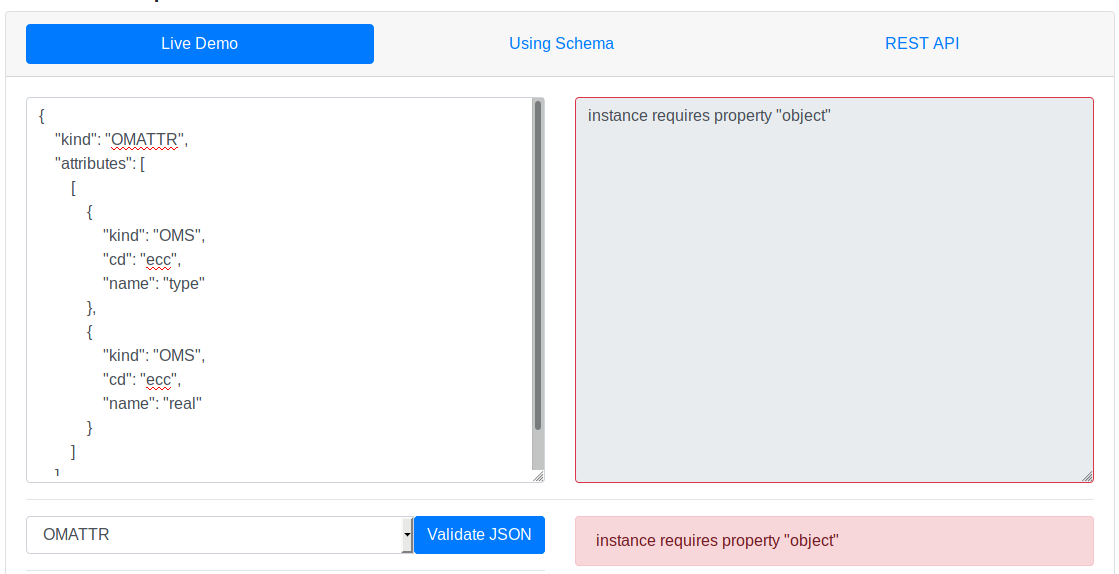
\includegraphics[width=\textwidth]{images/validate}
    \caption{Interface for validating an OpenMath object. }
    \label{figure:validate}
\end{figure}
Secondly, it enables validation of OpenMath JSON objects. This can be seen in Figure~\ref{figure:validate}.
The user can enter some JSON, press the \textit{Validate JSON} button, and receive immediate feedback if their JSON is a valid OpenMath object or not. 
In particular, the user can also see a detailed error message if their object is not valid OpenMath JSON. 

This makes use of the OpenMath JSON schema, and validates the users' JSON using a generic JSON Schema Validator. 
Furthermore, this is also exposed using a REST API, enabling easy validation of OpenMath JSON in other applications. 

\begin{figure}
    \centering
        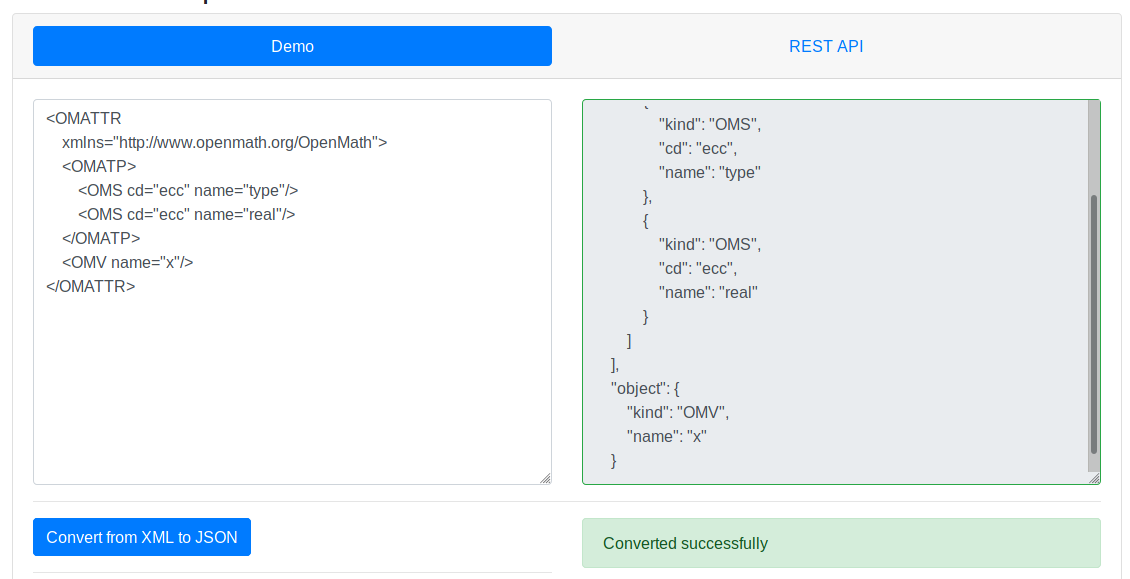
\includegraphics[width=\textwidth]{images/xml2json}
    \caption{Interface for converting OpenMath XML to JSON. }
    \label{figure:xml2json}
\end{figure}

\begin{figure}
    \centering
        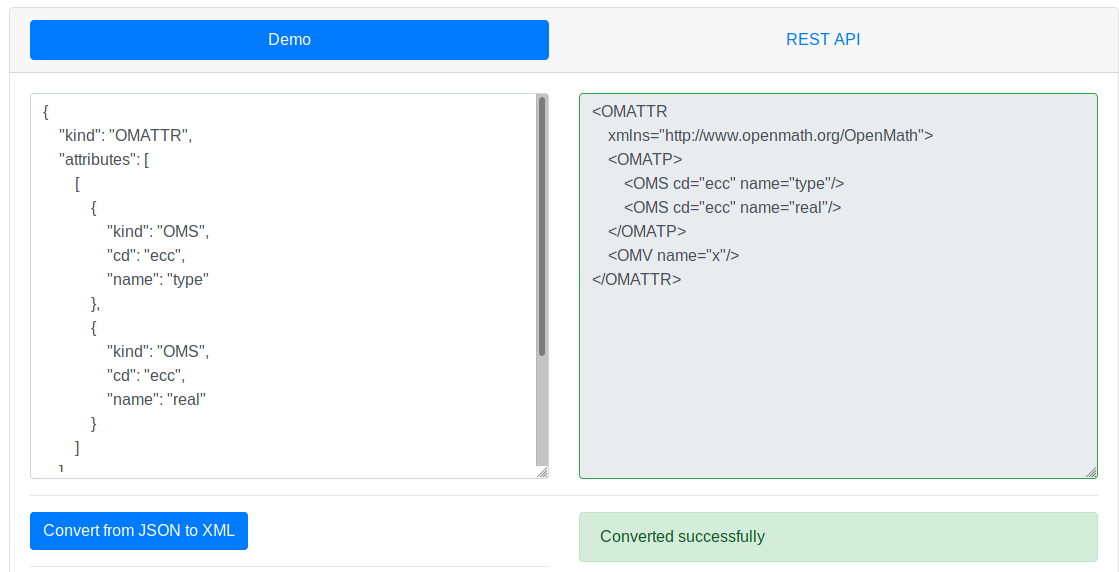
\includegraphics[width=\textwidth]{images/json2xml}
    \caption{Interface for converting OpenMath JSON to XML. }
    \label{figure:json2xml}
\end{figure}

Thirdly, it enables translation between XML and JSON OpenMath objects. 
Like for validation, the site enables the user to enter some JSON and be presented with some XML and vice-versa. 
This can be seen in Figures~\ref{figure:xml2json} and \ref{figure:json2xml}. 

As we designed our encoding with this translatability goal in mind, the implementation of it was straight-forward. 
Nonetheless, this translation is also exposed using a REST API. 

%  LocalWords:  handrewsjsonschema:18 vega-ts-jscon-schema-generator:webpage linewidth
%  LocalWords:  texttt textit textit subsubsection omel transc1 Hexademical attvar
%  LocalWords:  underbracket overbracket openmathjson:web centering includegraphics
%  LocalWords:  textwidth xml2json json2xml

    \section{Conclusion}

In this paper we have established that an OpenMath JSON encoding enables using OpenMath in many programming languages. 
The existing approaches for such an encoding did not make use of many of the native JSON features, hence we have developed our own encoding. 
This encoding is both easily translatable to and from the JSON encoding and makes use of native JSON features. 

\ednote{Not sure what else to write here}

    \printbibliography
\end{document}
